\documentclass[11pt]{article}
\usepackage{../../ee16}
\usepackage{../../markup}
\usepackage{tikz}
\usetikzlibrary{calc,shapes.geometric,arrows,automata}
\usepackage{color,hyperref,listings,enumitem}
\usepackage{algorithm}
\usepackage{algpseudocode}
\usepackage{tkz-euclide}
\usepackage{physics}
\usepackage{pgfplots}
\usepackage[american,siunitx]{circuitikz}
\lstset{basicstyle=\ttfamily}
\newcommand{\fillin}[1]{\underline{\hskip #1}}
\newcommand{\doublehrule}{\hrule \vskip 0.02in \hrule}
\newcommand*\circled[1]{\tikz[baseline=(char.base)]{`'
  \node[shape=circle,draw,inner sep=2pt] (char) {#1};}}
 
\newcommand{\sol}[1]{{\color{blue} \textbf{Meta: } #1}} % solutions in blue
\newcommand{\meta}[1]{{\color{blue} \textbf{Meta: } #1}}
%\newcommand{\sol}[1]{} % no solution sketches

\definecolor{blueish}{rgb}{0.7,0.1,.7}
%\newcommand{\ans}[1]{} % no numeric solutions
\newcommand{\ans}[1]{{\color{blueish} \textbf{Answer: } #1}} % numeric solutions

%\newcommand{\solans}[1]{}
\newcommand{\solans}[1]{{\color{blueish} \textbf{Answer: } #1}} %appears in both; use with caution

\usepackage{float}

\begin{document}

\def\title{Worksheet 8}

\maketitle

\vspace{0.5em}
% Lydia Lee, Spring 2019, lydia.lee@berkeley.edu
% \sol{
\qns{Review: Comparators}

Operational amplifiers (op amps for short) are typically drawn like the figure on the left, and their internal workings can be represented by the figure on the right.

\begin{minipage}{0.45\linewidth}
\begin{center}
  \begin{circuitikz}
    \draw (0,0) node[op amp,yscale=-1] (opamp) { }
      (-2.5, 0.5) to [short, i=$i_{+}$, o-] (opamp.+) 
      (-2.5, -0.5) to [short, i=$i_{-}$, o-] (opamp.-) 
      (opamp.out) node[right ] {$U_{out}$} 
      ;
    \node[draw=none,text=black] at (-2.8, 0.5) {$u_{+}$};
    \node[draw=none,text=black] at (-2.8, -0.5) {$u_{-}$};

    \draw (0, 0.5) to [short, -o] (0, 1.0);
    \node[draw=none,text=black] at (0, 1.5) {$V_{DD}$};
    \draw (0, -0.5) to [short, -o] (0, -1.0);
    \node[draw=none,text=black] at (0, -1.5) {$V_{SS}$};
  \end{circuitikz}
\end{center}
\end{minipage}
\begin{minipage}{.45\linewidth}
  \begin{center}
    % \textcolor{red}{This diagram may change slightly from semester to semester. We should stay consistent with the course notes to not confuse students.}
    \begin{circuitikz}
      % Nodes on the left
      \node[draw=none,text=black] at (-1, 0.8) {$u_{+}$};
      \node[draw=none,text=black] at (-1, -0.8) {$u_{-}$};
      \node[draw=none,text=black] at (-.8, 0.3) {$+$};
      \node[draw=none,text=black] at (-.8, -0.3) {$-$};
      \draw (-1.5, 0.5) to [short, -o] (-1, 0.5); 
      \draw (-1.5, -0.5) to [short, -o] (-1, -0.5); 
      
      % ground and variable voltage
      \draw (0.5,-1.5) -- (0.5,-1.8) to [short, -o](0.5, -2);
      \node[draw=none,text=black] at (1, -2) {$V_{SS}$};
      \draw (0.5, -1.5) -- (1, -1) -- (0.5, -0.5) -- (0, -1) -- cycle;
      \node[draw=none,text=black] at (0.5, -0.8) {$+$};
      \node[draw=none,text=black] at (0.5, -1.2) {$-$};
      \node[draw=none,text=black] at (1.8, -1) {$\frac{V_{DD}-V_{SS}}{2}$};
      \draw (0.5, -0.5) -- (0.5, 0) { };
      \draw (0.5, 0) -- (1, 0.5) -- (0.5, 1) -- (0, .5) -- cycle;
      \node[draw=none,text=black] at (0.5, 0.7) {$+$};
      \node[draw=none,text=black] at (0.5, 0.3) {$-$};
      \node[draw=none,text=black] at (2, 0.5) {$A(u_{+} - u_{-})$};
      
      % Upwards
      \draw (0.5, 1) -- (0.5, 1.5) to [short, -o] (3.5, 1.5);
      \draw (3.5,-1.5) to [short, o-] (3.5,-1.8) node[ground]{ };
      \node[draw=none,text=black] at (3.5, 1.8) {$U_{out}$};
      \node[draw=none,text=black] at (3.9, 1) {$+$};
      \node[draw=none,text=black] at (3.9, -1.6) {$-$};
    \end{circuitikz}
  \end{center} 
\end{minipage}

Here, $u_+$ and $u_-$ (both potentials) are input signals, $V_{DD}$ and $V_{SS}$ are what we call the ``supply rails'', and $U_{out}$ (a potential) is the output signal. From the diagram and knowing that $U_{out}$ cannot exceed the supply rail voltages, we have a relationship between the outputs and the inputs:
\begin{equation*}
U_{out} =
\begin{cases} 
V_{SS} &  
\hspace{1.4cm}A(u_+ - u_-) + \frac{V_{DD} +V_{SS} }{2} < V_{SS} \\
A(u_+ - u_-) + \frac{V_{DD} +V_{SS} }{2} & 
\hspace{0.4cm}V_{SS}\leq A(u_+ - u_-) + \frac{V_{DD} +V_{SS} }{2} \leq V_{DD} \\
V_{DD} &  
\hspace{0.4cm}V_{DD}<A(u_+ - u_-) + \frac{V_{DD} +V_{SS} }{2} \\
\end{cases}
\end{equation*}

\begin{center}
\begin{tikzpicture}
  \begin{axis}[
    xmin=-120, xmax=120,
    ymin=-120, ymax=120,
    axis lines=center,
    axis on top=true,
    grid style={dashed},
    xlabel={\emph{$u_{+} - u_{-}$}},
    ylabel={\emph{$U_{out}$}},
    yticklabels={,,},
    xticklabels={,,},
  ]
  \addplot [draw=blue,thick] coordinates {(5, 70) (100, 70)};
  \addplot [draw=blue,thick] coordinates {(-5, -20) (-100, -20)};
  \addplot [draw=blue,thick] coordinates {(-5, -20) (5, 70)};
  \addplot [
      mark=*, blue, solid
    ]
    coordinates {
            (-5, -20)
            (5, 70)};

    \node[anchor=north west] at (axis cs:-5,-20) {$(0,V_{SS})$};
    \node[anchor=south east] at (axis cs:5,70) {$(0,V_{DD})$};
  \end{axis}
\end{tikzpicture}
\end{center}

Typically $A$ is quite large, meaning the the sloped region in the center is quite narrow. This is particularly useful when comparing two voltages (hence, the name \textit{comparator}), one or both of which may be variable.
% }
\empt{\newpage}
% Lydia Lee, adapted from Fall 2018 notes
% \sol{
\qns{Review: Negative Feedback}

The classic formulation of the negative feedback problem looks like so:
\begin{figure}[H]
	\centering
	\tikzstyle{block} = [draw, fill=white, rectangle, 
      minimum height=3em, minimum width=3em]
	\tikzstyle{sum} = [draw, fill=white, circle, node distance=1cm]
	\tikzstyle{input} = [coordinate]
	\tikzstyle{output} = [coordinate]
	\tikzstyle{midoutput} = [coordinate]
	\tikzstyle{pinstyle} = [pin edge={to-,thin,black}]
	\begin{tikzpicture}[auto, node distance=2cm,>=latex']
    % We start by placing the blocks
    \node [input, label=$s_\text{in}$] (input) {$s_\text{in}$};
    \node [sum, right of=input] (sum) { };
    \node [block, right of=sum] (gain) {$A$};
    % \node [midoutput, right of=gain] (midoutput) {};
    \node [output, right of=gain, label=$s_\text{out}$] (output) {$s_\text{out}$};
    % \draw [->] (gain) -- node[name=u] (output) {output} ;
    \node [block, below of=gain] (F) {$f$};
      
   % Once the nodes are placed, connecting them is easy. 
    \draw [draw,->] (input) -- node[pos=0.85] {$+$} node [near end] {} (sum);
   \draw [->] (sum) -- node {$s_\text{error}$} (gain);
   \draw [->] (gain) -- node [name=y] {} (output);
   \draw [->] (y) |- (F);
   \draw [->] (F) -| node[pos=0.99] {$-$} node [near end] {$s_\text{fb}$} (sum);
  \end{tikzpicture}
	\label{fig:nfb_block_diagram}
	\caption{Classic negative feedback block diagram}
\end{figure}
For the block diagram above, the output is related to the input by 
\begin{align*}
	s_\text{out} &= \frac{A}{1+Af}s_\text{in}\\
		&\approx \frac{1}{f} \text{ when }A\to\infty
\end{align*}
In this class, the block for $A$  often involves the use of an operational amplifier, or op amp (not to be confused with OMP!) for short. For these situations, the value of $A\to\infty$, so we can make some assumptions known as the ``Golden Rules''.
\begin{itemize}
	\item Always true: $i_- = i_+ = 0\si{\ampere}$
	\item Negative feedback only: $u_+ = u_-$
\end{itemize}
\sol{
\begin{center}
  \begin{circuitikz}
    \draw (0,0) node[op amp,yscale=-1] (opamp) { }
      (-2.5, 0.5) to [short, i=$i_{+}$, o-] (opamp.+) 
      (-2.5, -0.5) to [short, i=$i_{-}$, o-] (opamp.-) 
      (opamp.out) node[right ] {$U_{out}$} 
      ;
    \node[draw=none,text=black] at (-2.8, 0.5) {$u_{+}$};
    \node[draw=none,text=black] at (-2.8, -0.5) {$u_{-}$};

    \draw (0, 0.5) to [short, -o] (0, 1.0);
    \node[draw=none,text=black] at (0, 1.5) {$V_{DD}$};
    \draw (0, -0.5) to [short, -o] (0, -1.0);
    \node[draw=none,text=black] at (0, -1.5) {$V_{SS}$};
  \end{circuitikz}
\end{center}

When dealing with feedback topologies, we often want to know two things:
\begin{itemize}
	\item Is it actually in negative feedback?
	\item What is the relationship of the output signal with respect to the input signal?
\end{itemize}
}

The way we show that a system is in negative feedback involves a bit of a gedankenexperiment\footnote{\url{https://en.wikipedia.org/wiki/Thought_experiment}}.
\begin{enumerate}
	\item Turn off all independent sources
	\item Perturb the output by pretending that it gets ``kicked'' up (or down)
	\item Go around the feedback loop to see how the inputs of the op amp $u_+$ and $u_-$ are affected (i.e. do they go up or down?)
	\item After determining how the inputs of the op amp responds to the initial stimulus, see how the output of the amp responds to the changing op amp inputs. If the system is in negative feedback, the output should be pushed in the \textit{opposite} direction as the initial stimulus! 
\end{enumerate}

\textbf{Side-Note:}
The notion of negative feedback converging to a single stable point is analogous to a ball being at the bottom of a valley. If you push the ball left or right (analogous to ``kicking'' the output), the ball will always settle back to that stable point. The notion of electrical potential is directly analogous to mechanical potential.
\empt{\newpage}
% }

\begin{qunlist}
% Author: Varsha Ramakrishnan
% Email:vio@berkeley.edu

\qns{Capacitive Touchscreen}

\sol{Prereq: Ability to solve capacitor equivalences.}



Consider the following capacitive touchscreen configuration. (This is a review from lecture.)

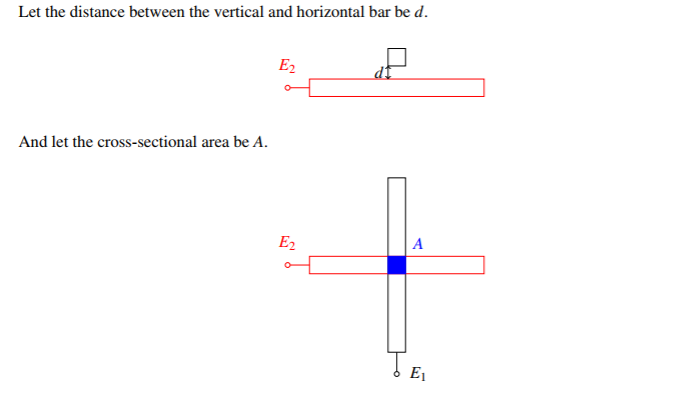
\includegraphics{questions/capacitors.png}

\begin{enumerate}
\qitem{
Draw a diagram representing the capacitance between $E_1$ and $E_2$ when there is no touch on the screen.
}

\ans{

\begin{center}
\begin{circuitikz}
\draw(0,0) 
    to[short, -o, l=$E_1$] ++(0, 0);
\draw(0,0)
	to[C=$C_1$] ++(0,2)
	to[short, -o, l=$E_2$] ++(0,0);

\end{circuitikz}
\end{center}
}

\qitem {
Calculate the value of the capacitance between the two bars when the screen is not being touched.
}
\ans{
$$C_1 = \epsilon A/d$$
}

\qitem{
	Now consider what happens when we touch the screen. Let the blue line represent our finger, and assume there is a capacitance between your finger and each of the bars. The diagram looks like this:
	
	\begin{center}
	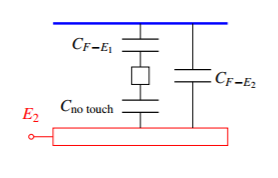
\includegraphics{questions/capacitors_touch.png}
    \end{center}
    Redraw the circuit diagram representing the capacitive touchscreen after being touched, so that the nodes representing $E_1$ and $E_2$ are on opposite ends of the diagram.
    
\begin{center}
\begin{circuitikz}

	
\draw(0,0)
    to[short, -o, l=$E_2$] ++(0, -1);

\draw(0,4)
    to[short, -o, l=$E_1$] ++(0, 1);

\end{circuitikz}
\end{center}
    
}

\ans{
\begin{center}
\begin{circuitikz}
\draw(0,0) 
	to[short] ++(3,0)
	to[C=$C_{F-E_2}$] ++(0,2)
	to node[right] {$\gets$ Finger} ++(0,0)
	to[C=$C_{F-E_1}$] ++(0,2)
	to[short] ++(-3,0)
	to[C=$C_{no\ touch}$] ++(0,-4);
	
\draw(0,0)
    to[short, -o, l=$E_2$] ++(0, -1);

\draw(0,4)
    to[short, -o, l=$E_1$] ++(0, 1);

\end{circuitikz}
\end{center}
}

\qitem{Calculate the new capacitance between $E_1$ and $E_2$. Has it changed from when there was no touch?}

\ans{
Begin by writing the equation that relates all the capacitors using parallel and series symbols, then expand:
\begin{align*}
C_{E_1-E_2}  &= C_{no\ touch} + C_{F-E_1} || C_{F-E_2} \\
&= C_{no\ touch} + \frac{C_{F-E_1}C_{F-E_2}}{C_{F-E_1} + C_{F-E_2}}
\end{align*}
The new capacitance (after touch) is larger than the previous capacitance (before touch). Since the capacitance value has changed by a measurable amount, we can work backwards and find the distance at which the screen was touched.
}


\end{enumerate}
% Author: Henry Sun, Rohan Suresh, Sukrit Arora
% Email: tigerhs1998@berkeley.edu, rohansuresh@berkeley.edu


\qns{OpAmps as Comparators}
\begin{enumerate}
\qitem{Now you've learned about a new component, the operational amplifier. What can this circuit component be used for? How does it work?}

\ans{
This component can be used to compare two inputs, amplify the output of an input, or act as a buffer in the middle of a circuit.
}

\begin{circuitikz} \draw
(0,0) node[op amp, yscale=-1] (opamp) {}
(opamp.-) node[left] {$v_-$}
(opamp.+) node[left] {$v_+$}
(opamp.out) node[right] {$v_o$}
(opamp.down) --++(0,0.5) node[vcc]{$V_{DD}$}
(opamp.up) --++(0,-0.5) node[vee]{$V_{SS}$}
;\end{circuitikz}
\qitem{
Above we have the basic schematic of the op-amp. What does each terminal mean? How do we determine the output voltage? Are there any constraints?
}
\empt{
\vspace{2cm}
}
\ans{
The $V_+$ and $V_-$ are the input terminals to the op-amp. The $V_{DD}$ and $V_{SS}$ are what power the op-amp, and are the values that the comparator will output. Finally $V_o$ is what the op-amp outputs, which is defined as $A(V_+-V_-)$ where $A$ is some large gain value.
}

\qitem{
Much of EE16A will have our analysis be restricted to ideal op-amps. However, it is important to know non-ideal behaviors. What are some main differences between ideal and non-ideal op-amps?
}
\empt{
\vspace{1.5cm}
}
\ans{
Ideal op-amps: Infinite gain $A = \frac{V_o}{V_i}$ (where $V_i = V_+ - V_-$). This means that the gain will be infinity if there was no limit on the rails, but it cannot reach infinity because it gets clipped at the positive or negative rails. infinite input resistance, zero input current. Non-ideal op amps: finite gain, finite input resistance, finite input current.
}

\qitem{
Below are some op-amp configurations. Please identify the output voltage $V_o$ for each.

\begin{enumerate}
\item{
\begin{circuitikz} \draw
(0,0) node[op amp, yscale=-1] (opamp) {}
(opamp.-) node[left] {10V}
(opamp.+) node[left] {5V}
(opamp.out) node[right] {$v_o$}
(opamp.down) --++(0,0.5) node[vcc]{20V}
(opamp.up) --++(0,-0.5) node[vee]{-20V}
;\end{circuitikz}
}
\item{
\begin{circuitikz} \draw
(0,0) node[op amp, yscale=-1] (opamp) {}
(opamp.-) node[left] {$v_-$}
(opamp.+) node[left] {$v_+$}
(opamp.out) node[right] {$v_o$}
(opamp.down) --++(0,0.5) node[vcc]{$V_{DD}$}
(opamp.up) --++(0,-0.5) node[vee]{$V_{SS}$}
;\end{circuitikz}
}

\end{enumerate}
}

\ans{
\newline
i. $V_o = -20V$
\newline
ii. $V_o = V_{DD}$ if $V_+ > V_-$, $V_o = V_{SS}$ if $V_- > V_+$
}

\end{enumerate}
\empt{\newpage}
\end{qunlist}

\end{document}

